\documentclass[11pt]{article}
% Overleaf-ready draft. Swap \documentclass for the workshop style when chosen.
\usepackage[margin=1in]{geometry}
\usepackage{graphicx}
\usepackage{booktabs}
\usepackage{array}
\usepackage{amsmath}
\usepackage[hidelinks]{hyperref}
\usepackage{xcolor}
\usepackage{authblk}

\title{Incidental Visual Affect Shifts the Behavior of Vision--Language Models}
\author[1]{Charlotte Li}
\author[1]{Arnav (halli75)}
\author[1]{Algoverse 2026 team}
\affil[1]{Algoverse AI Research}
\date{Draft --- \today}

% Provenance tags for every empirical claim:
\newcommand{\srcA}{\textcolor{orange!80!black}{[A]}} % Arnav's run: gemma-4-E4B, github.com/halli75/Algoverse
\newcommand{\srcM}{\textcolor{blue!70!black}{[M]}}    % this work: multi-model sweep (pikanaeri/affect-control-axis)

\begin{document}
\maketitle

\begin{abstract}
Vision--language models (VLMs) are routinely shown images that are irrelevant to the task at hand. We ask whether such \emph{incidental} affective imagery systematically changes a VLM's decisions. Prepending a task-irrelevant emotional image to established decision paradigms, and measuring behavior generation-free (first-token option-logits), we find that a photo raises benign over-refusal from ${\sim}66\text{--}80\%$ to ${\sim}92\text{--}97\%$ across two model families, and that the \emph{image} channel shifts behavior in a way matched text captions do not reproduce (a cross-modal dissociation), while leaving plain capability intact. A white-box analysis in Gemma-3-12B identifies an internal affect direction, shared between image and text, whose activation causally gates this behavior. Discrete fear-vs-anger contrasts are null, consistent with a dimensional (valence) rather than categorical account. We frame this as a controllability and robustness property of deployed multimodal systems.
\end{abstract}

\paragraph{Provenance.} This draft combines two runs, tagged throughout: \srcA{}~= the original battery run by Arnav (halli75) on \texttt{google/gemma-4-E4B-it} (\url{https://github.com/halli75/Algoverse}), and \srcM{}~= this work's multi-model replication and extension across five VLMs (\url{https://github.com/pikanaeri/affect-control-axis}). Where both ran an experiment, we report \srcA{} for the original documented effect size and \srcM{} for the cross-model replication. All behavior is generation-free; only existing benchmarks are used; no crafted attacks are released.

\section{Introduction}
\emph{[Stub.]} Deployed VLMs perceive incidental imagery constantly. If a task-irrelevant affective image silently re-weights the model's decisions, that is an alignment-relevant robustness issue. We test this across cognitive, social, epistemic, and safety-calibration paradigms and multiple model families, and connect the behavioral effect to an internal affect representation.

\section{Related Work}
\emph{[Stub; see \texttt{docs/NOVELTY\_SEARCH.md}.]} Prior work separately shows that visual primes can influence VLM outputs, that textual/internal emotional manipulations alter LLM behavior, and that emotional context can affect agents. We connect these: whether \emph{task-irrelevant, naturalistic visual affect} induces structured, cross-model behavioral change, decomposed by valence/arousal/dominance vs.\ discrete emotion, and mechanistically mediated by a shared affect direction.

\section{Methods}
\paragraph{Models.} Five instruction-tuned VLMs across two families and 2--12B: Gemma-4-E4B, Gemma-4-12B, and Qwen3-VL-2B/-4B/-9B, loaded in 4-bit (nf4) weights, bf16 compute. White-box analysis additionally uses Gemma-3-12B.
\paragraph{Stimuli.} EMOTIC (natural images, 26 discrete emotion categories + continuous valence/arousal/dominance; fixed eval split) prepended with chat order \texttt{[image, text]}; the prompt never refers to the image. OASIS (viewer-elicited valence/arousal) is used for the image-derived affect axis and the depicted-vs-elicited contrast. Images are capped at 512\,px.
\paragraph{Metric.} Every decision is a first-token option-logit: $\mathrm{logsumexp}(\text{A})-\mathrm{logsumexp}(\text{B})$ at the answer position --- a tendency, no generation, no judge. Effects are $\Delta$ vs.\ a neutral/no-image baseline with bootstrap 95\% CIs (an effect is present iff the CI excludes 0).
\paragraph{White-box mechanism.} A per-layer affect direction $a$ (diff-in-means of low- vs.\ high-valence residuals) is intervened on by norm-scaled steering ($\Delta = \alpha\,\lVert h\rVert\,\hat a$), with a random-direction control, coherence gate, massive-activation removal, and split-half stability; causal mediation is tested by steer-and-restore.

\subsection{Emotions used}
The battery draws EMOTIC categories chosen to span the affective space, plus a no-image baseline (Table~\ref{tab:emotions}). The white-box spectrum analysis (extension) additionally uses Excitement.

\begin{table}[h]\centering\small
\begin{tabular}{lccc}
\toprule
Emotion & Valence & Arousal & Used in \\
\midrule
Fear & $-$ & high & exp01, exp06, exp09 \\
Anger & $-$ & high & exp01, exp05, exp06, exp09 \\
Sadness & $-$ & low & exp06, exp09 \\
Happiness & $+$ & high & exp05, exp06, exp09 \\
Peace & $+$ & low & exp06, exp09 \\
Affection & $+$ & mid & exp05 \\
Neutral & $\approx$ & low & exp06, exp09 (control) \\
\emph{no-image} & --- & --- & baseline (all) \\
\bottomrule
\end{tabular}
\caption{Affective image conditions used in the behavioral battery. (Excitement is added in the white-box emotion-spectrum extension.)}
\label{tab:emotions}
\end{table}

\section{Results}

\subsection{An internal affect axis causally shifts behavior (white-box) \srcM}
In Gemma-3-12B, steering the affect axis toward benign collapses refusal along a clean dose-response ($1.00\to0.00$) while a matched random direction stays pinned at $1.00$; restoring the projection onto the refusal direction recovers refusal fully ($0.25\to1.00$), so the effect is routed through that direction. Images reach the axis $\sim$15--23\% of a full steer in a neutral/task context but only $\sim$0.7\% under a harmful prompt --- images cannot jailbreak refusal but can move softer behavior.

\subsection{Over-refusal rises across model families \srcM}
A task-irrelevant photo (any category, including neutral) sharply raises benign over-refusal on XSTest (exp09), with non-overlapping CIs and an identical direction across families (Figure~\ref{fig:overrefusal}): Gemma-4-E4B $0.66\to0.92$, Qwen3-VL-2B $0.71\to0.97$, Qwen3-VL-4B $0.80\to0.96$. The original run reported the same shift on Gemma-4-E4B ($\sim$66\%$\to$91--94\%) \srcA. This is a global caution shift, not improved safety reasoning.

\begin{figure}[h]\centering
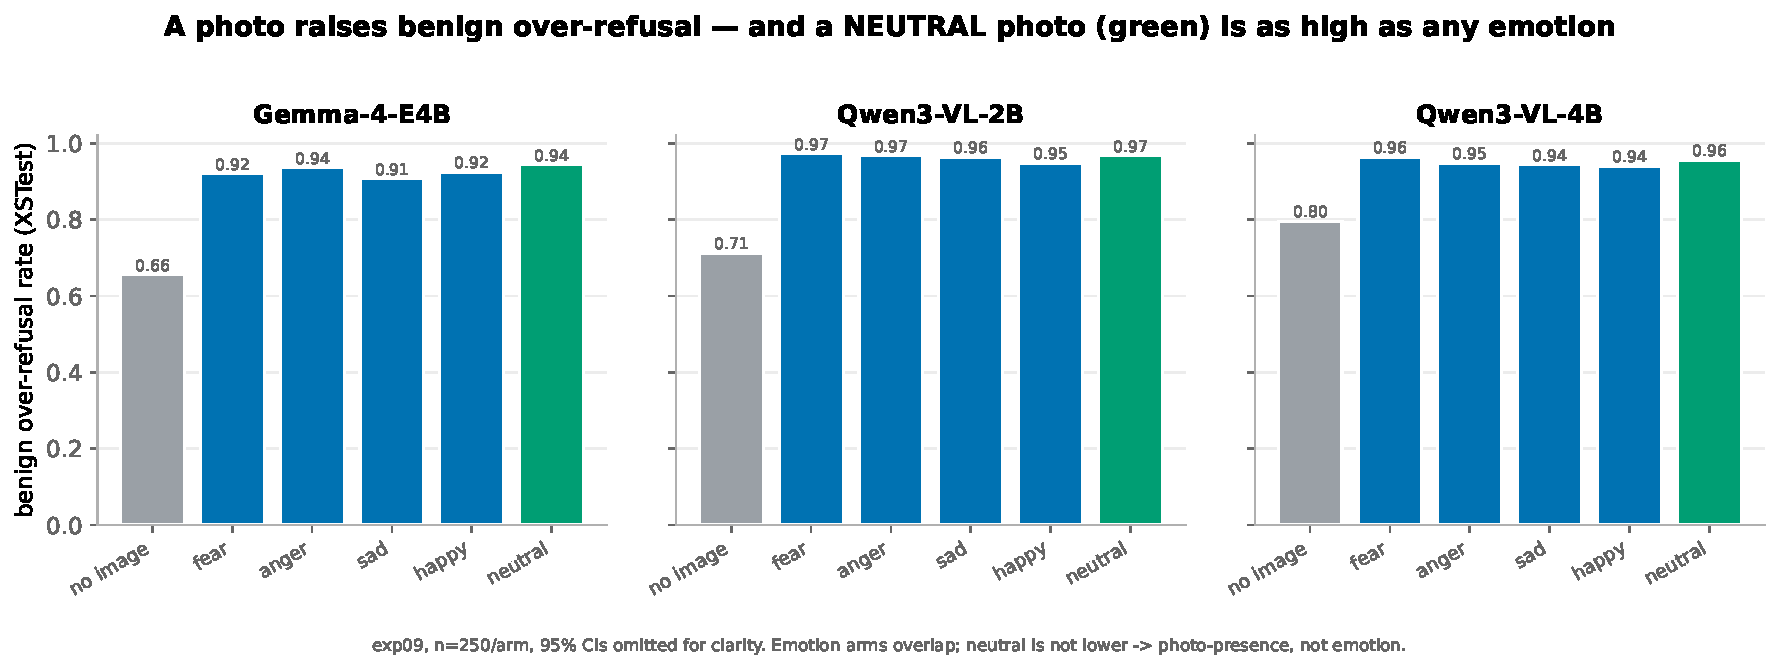
\includegraphics[width=0.72\linewidth]{figures/fig1_overrefusal_crossmodel.pdf}
\caption{Over-refusal (exp09) after an unrelated photo, across three VLMs. Error bars are 95\% CIs ($n=250$/condition). \srcM}
\label{fig:overrefusal}
\end{figure}

\subsection{The image channel shifts behavior; matched text does not \srcA\srcM}
On Gemma-4-E4B (exp03, \texttt{CROSS\_MODAL\_DIVERGE}, gates 9/9), the \emph{photo} moves generosity/behavior --- $\mathrm{dictator{:}pixels}=-0.98\,[-1.97,-0.19]$ \srcA{} and $\mathrm{perez{:}pixels}=-0.69\,[-1.23,-0.09]$ \srcM{} --- while matched captions, emotion labels, and narratives do not copy it (Figure~\ref{fig:crossmodal}). Qwen3-VL-2B shows the same image-channel signal ($\mathrm{risk{:}deaffect}=+0.80\,[+0.06,+1.55]$; $\mathrm{dictator{:}label}=-1.12\,[-2.09,-0.19]$) \srcM. The model is not simply reading an emotion word off the picture.

\begin{figure}[h]\centering
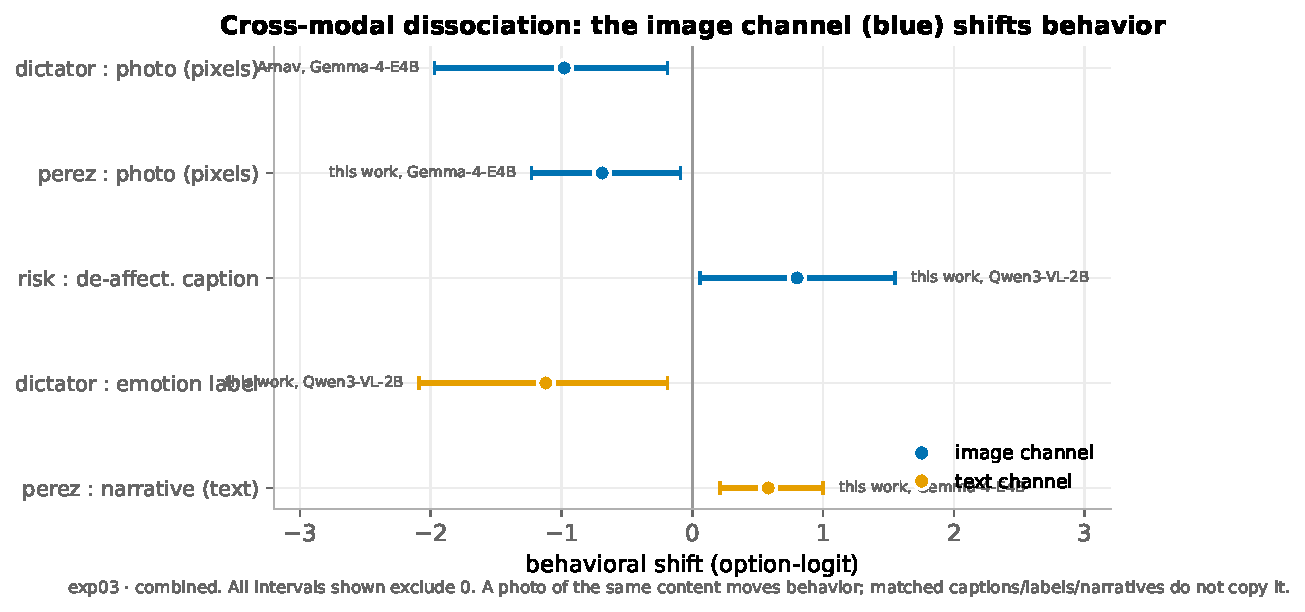
\includegraphics[width=0.82\linewidth]{figures/fig2_crossmodal_dissociation.pdf}
\caption{Cross-modal dissociation (exp03): image-channel effects (blue) vs.\ text-channel (orange). All intervals shown exclude 0. \srcA\srcM}
\label{fig:crossmodal}
\end{figure}

\subsection{Specificity and controls}
Discrete fear-vs-anger on risky lotteries is null ($\Delta\approx-0.09$, CI includes 0) \srcA\srcM, pointing away from categorical and toward a valence account. A capability control (exp07) shows accuracy flat at $\sim$0.68--0.72 across affect conditions \srcA\srcM{} --- affect does not degrade knowledge, so the behavioral effects are not generic distraction.

\subsection{Full battery}
Table~\ref{tab:battery} summarizes all ten experiments, their outcome, result, analysis, and source.

\begin{table}[h]\centering\footnotesize
\renewcommand{\arraystretch}{1.25}
\begin{tabular}{@{}l l c p{4.3cm} p{3.6cm} c@{}}
\toprule
Exp & Construct & Outcome & Result & Analysis & Src \\
\midrule
exp01 & Risk (fear vs anger) & Null & $\Delta\approx-0.09$, CI incl.\ 0 & No discrete-emotion effect; supports valence account & A,M \\
exp02 & Scene-matched control & Null & No exp01 effect to explain & Downstream of a null & A,M \\
exp03 & Cross-modal + generosity & \textbf{Success} & Photo moves behavior ($-0.98$\,\srcA, $-0.69$\,\srcM); text does not & Image channel $\neq$ text & A,M \\
exp04 & Sycophancy (Perez) & Null & Behavioral-delta only; mean $\Delta$ incl.\ 0 & No reliable sycophancy shift & A,M \\
exp05 & Fairness / generosity & Partial & Anger $\to$ more unfair-reject \srcA; small dictator shifts \srcM & Punishment up; giving weak & A,M \\
exp06 & Patience (discounting) & \emph{Excluded} & Degenerate $k$-estimator (identical across conditions) & Estimator bug, not a result & A,M \\
exp07 & Capability (control) & Null (good) & Accuracy $\sim$0.68--0.72, flat & Affect does not degrade knowledge & A,M \\
exp08 & Stimulus (EMOTIC/OASIS) & Mixed & Signatures match \srcM; both-null \srcA & Shared construct; do not pool & A,M \\
exp09 & Over-refusal (XSTest) & \textbf{Success} & $\sim$66--80\% $\to$ 92--97\%, three models & Global caution shift, cross-family & A,M \\
exp10 & Mediation & Partial & \texttt{DIAGNOSTIC\_NOT\_V3}; risk shift, correlational mediation & Consistent, not causal mediation & A,M \\
\bottomrule
\end{tabular}
\caption{The behavioral battery. Outcome is the scientific label (did we see a difference worth reporting), not ``did the job finish.'' Src: \srcA{}~Arnav (Gemma-4-E4B), \srcM{}~this work (multi-model). Original verdicts are exploratory (smoke tier, no pre-registration).}
\label{tab:battery}
\end{table}

\section{Discussion}
\emph{[Stub.]} Incidental visual affect acts as a latent control signal on VLM behavior: the most reliable manifestation is a global caution shift (over-refusal), the effect enters through the image channel rather than emotion words, and it is carried by a continuous valence dimension. This is a controllability property with a defensive reading --- the same axis that carries the effect is a clean monitor.

\section{Limitations and Ethics}
Battery numbers are exploratory (smoke tier, small $n$; exp03 $n=8$); the headline effects warrant a pre-registered, full-tier rerun. exp06 is excluded (estimator bug). The 12B/9B models OOM'd on the image-heavy experiments, so the cross-model claim rests on three 4B-class models across two families; the refusal \emph{gate} is model-specific (Gemma-3-12B) and the paper is anchored on the behavioral results. Ethics: refusal is measured generation-free; only existing benchmarks (AdvBench, Alpaca, XSTest, TruthfulQA/MMLU, EMOTIC, OASIS) are used; agentic scenarios are hypothetical decision framings scored by option-logit (a tendency, not executed actions); no harmful completions are stored (aggregate rates only) and no crafted attacks are released.

\end{document}
